\documentclass[12pt]{article}

\usepackage{amsmath,amsthm,amsfonts,amssymb,amsxtra}
\usepackage{pgf,tikz}
\usetikzlibrary{arrows}
\renewcommand{\theenumi}{(\alph{enumi})} 
\renewcommand{\labelenumi}{\theenumi}

\pagestyle{empty}
\setlength{\textwidth}{7in}
\setlength{\oddsidemargin}{-0.5in}
\setlength{\topmargin}{-1.0in}
\setlength{\textheight}{9.5in}

\newtheorem{problem}{Problem}

\begin{document}

\noindent{\large\bf MATH 141}\hfill{\large\bf Exam\#3.}\hfill{\large\bf
  Fall 2009}\hfill{\large\bf Page 1/5}\hrule

\bigskip
\begin{center}
  \begin{tabular}{|ll|}
    \hline & \cr
    {\bf Name: } & \makebox[12cm]{\hrulefill}\cr & \cr
    {\bf 4-digit code:} & \makebox[12cm]{\hrulefill}\cr & \cr
    \hline
  \end{tabular}
\end{center}
\begin{itemize}
\item Write your name and the last 4 digits of your SSN in the space provided above.
\item The test has five (5) pages, including this one.
\item Enter your answer in the box(es) provided.
\item You must show sufficient work to justify all answers unless
  otherwise stated in the problem.  Correct answers with inconsistent
  work may not be given credit.
\item Credit for each problem is given in parentheses at the right of
  the problem number.
\item No books, notes or calculators may be used on this test.
\end{itemize}
\hrule

\begin{center}
  \begin{tabular}{|c|c|c|}
    \hline
    &&\cr
    {\large\bf Page} & {\large\bf Max.~points} & {\large\bf Your points} \cr
    &&\cr
    \hline
    &&\cr
    {\Large 2} & \Large 30 & \cr
    &&\cr
    \hline
    &&\cr
    {\Large 3} & \Large 30 & \cr
    &&\cr
    \hline
    &&\cr
    {\Large 4} & \Large 20 & \cr
    &&\cr
    \hline
    &&\cr
    {\Large 5} & \Large 20 & \cr
    &&\cr
    \hline\hline
    &&\cr
    {\large\bf Total} & \Large 100 & \cr
    &&\cr
    \hline
  \end{tabular}
\end{center}
\newpage

%%%%%%%%%%%%%%%%%%%%%%%%%%%%%%%%%%%%% Page 2
\noindent{\large\bf MATH 141}\hfill{\large\bf Exam\#3.}\hfill{\large\bf
  Fall 2009}\hfill{\large\bf Page 2/5}\hrule

\bigskip
{\problem[30 pts] \em  Evaluate each integral:} 
\begin{enumerate}
\item $\displaystyle{\int \big( 3\sin x - 2\sec^2 x \big)\, dx}$
\vspace{6cm}
\item $\displaystyle{\int \frac{5x^4}{(x^5+1)^2}\, dx}$
\vspace{6cm}
\item $\displaystyle{\int_0^1 (5x-3)\, dx}$
\end{enumerate}
\newpage

%%%%%%%%%%%%%%%%%%%%%%%%%%%%%%%%%%%%% Page 3
\noindent{\large\bf MATH 141}\hfill{\large\bf Exam\#3.}\hfill{\large\bf
  Fall 2009}\hfill{\large\bf Page 3/5}\hrule

\bigskip
{\problem[20 pts] \em Express the following functions of $n$ in closed
  form and then find the limit.}
\begin{enumerate}
\item  $\displaystyle{\lim_{n \to \infty} \frac{1^2+2^2+3^2+ \dotsb +
      n^2}{n^3}}$
\vspace{5cm}
\item  $\displaystyle{\lim_{n \to \infty} \sum_{k=1}^n \frac{5k}{n^2}}$
\vspace{5cm}
\end{enumerate}
\hrule
{\problem[10 pts] \em Use the definition of \textbf{definite integral} to
  express $\int_{-\pi/2}^{\pi/2} (1+ \cos x)\, dx$ as a limit.}
\newpage

%%%%%%%%%%%%%%%%%%%%%%%%%%%%%%%%%%%%% Page 4
\noindent{\large\bf MATH 141}\hfill{\large\bf Exam\#3.}\hfill{\large\bf
  Fall 2009}\hfill{\large\bf Page 4/5}\hrule

\bigskip
{\problem[20 pts] \em Sketch the graph of the rational function $f(x)
  = \displaystyle{\frac{2x^2-8}{x^2-16}}$.}
\begin{quotation}
Use the back of this page for computations and sign-charts. Indicate clearly:
\begin{itemize}
\item Domain
\item $x$- and $y$-intercepts.
\item Vertical and horizontal asymptotes (any holes?).
\item Intervals of increase, decrease and different concavity.
\item Location of relative extrema and inflection points. 
\end{itemize}
\end{quotation}
\noindent\textbf{HINT:} The first and second derivatives are,
respectively 
\begin{equation*}
f'(x) = \frac{-48x}{(x^2-16)^2}, \quad f''(x) = 48 \frac{3x^2+16}{(x^2-16)^3}
\end{equation*}
\vspace{1cm}
\begin{center}
\begin{tikzpicture}
\draw[step=0.5cm, gray] (-0.25cm,-0.25cm) grid (12.25cm,12.25cm);
\draw[<->,very thick] (-0.5cm,6cm) -- (12.5cm,6cm);
\draw[<->,very thick] (6cm,-0.5cm) -- (6cm,12.5cm);
\end{tikzpicture}
\end{center}
\newpage

%%%%%%%%%%%%%%%%%%%%%%%%%%%%%%%%%%%%% Page 5
\noindent{\large\bf MATH 141}\hfill{\large\bf Exam\#3.}\hfill{\large\bf
  Fall 2009}\hfill{\large\bf Page 5/5}\hrule

\bigskip
{\problem[10 pts] \em Use the Fundamental Theorem of Calculus to find
  the derivative of the following functions.}
\begin{enumerate}
\item $\displaystyle{g(x) = \int_1^x \frac{1}{t^3+1}\, dt}$
\vspace{1cm}
\begin{flushright}
  \begin{tikzpicture}
    \draw (-1cm,2.5cm) node {$g'(x) =$};
    \draw (0cm,1.8cm) rectangle (5cm,3.2cm);
 \end{tikzpicture}
\end{flushright}
\item $\displaystyle{g(y) = \int_x^\pi \sqrt{1+ \sec t}\, dt}$
\vspace{1cm}
\begin{flushright}
  \begin{tikzpicture}
    \draw (-1cm,2.5cm) node {$g'(y) =$};
    \draw (0cm,1.8cm) rectangle (5cm,3.2cm);
 \end{tikzpicture}
\end{flushright}
\end{enumerate}
\hrule
{\problem[10 pts] \em Find the antiderivative $F$ of $f(x) =
  4-3(1+x^2)^{-1}$ that satisfies $F(1) = 0$.} 

\noindent\textbf{HINT:} You need to use the constant of integration.
\vspace{8cm}
\begin{flushright}
  \begin{tikzpicture}
    \draw (-1cm,2.5cm) node {$F(x) =$};
    \draw (0cm,1.8cm) rectangle (5cm,3.2cm);
 \end{tikzpicture}
\end{flushright}

\end{document}
